\chapter{Related Work}
\label{ch:relatedwork}

This chapter will describe two well-known data structures for static range searching: the kd-tree and the range tree. The kd-tree is the current de facto standard for static range searching because of its low space complexity. It has a space complexity of $\mathcal{O}(n)$ and a running time of $\mathcal{O}(\sqrt{n} + k)$ where $k$ is the number of results reported. In practise it uses the exact same amount of words as it holds elements\cite{compgeo}. The range tree uses $\mathcal{O}(n \lg n)$ words of space and has a running time of $\mathcal{O}(\lg^2 n + k)$ without \emph{fractional cascading} and a running time of $\mathcal{O}(\lg n + k)$ with fractional cascading. The difference between the space complexities of the kd-tree and the range tree is a factor $\mathcal{O}(\lg n)$ which can become an issue when dealing with very large datasets and a limited amount of main memory. This factor can grow big for large datasets and is the reason why kd-trees are prefered in practise.

The kd-tree will be used as a reference in the comparison against the Simple Range Search data structure since they have the same space complexity. This property makes the Simple Range Search data structure quite attractive. The range tree will be used to show how much the running time can be decreased by increasing the space complexity by a factor of $\mathcal{O}(\lg n)$. The range tree will also be used to introduce some of the ideas behind the Simple Range Search and Original Range Search data structures, which is where \citet{chanetal} drew some of their inspiration.

The query time of the main data structures in this chapter are all \emph{output-sensitive}, meaning that their running time depends on the amount of results found. The data structures themselves are static: After the initial construction of the data structures they will not be altered by insertions or deletions. \todo{more} 

\section{kd-trees}
\label{sect:kdtrees}

The current standard of range reporting using linear space is the kd-tree. This data structure will be used as a reference point when evaluting the results of the primary work of the thesis. With linear space it is a fitting data structure for range reporting on the RAM, and a practical solution. The kd-tree with $n$ points can be represented as an array $A[1..n]$.\todo{Beskriver det fint nok at størrelsen er $n$?}

\begin{figure}[h]
    \centering
    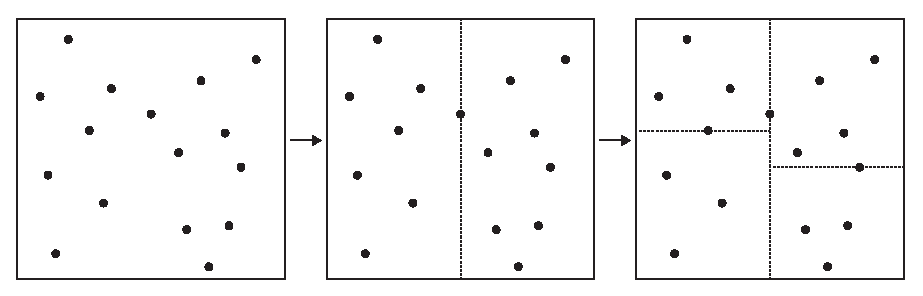
\includegraphics[width = 1.0\textwidth]{pictures/kd_subdivision.eps}
    \caption{Showing the subdivision of points in a node: First dividing the points by the x-median, and then by the y-median}\label{fig:kdsubdivision}
\end{figure}


A kd-tree is constructed recursively: Given $n$ points, the median of the points with respect to x is found. All points which has an x-coordinate larger than the median goes to the right child, while points which has an x-coordinate smaller than the median, and the median point, goes to the left child. At the next level the points of each node will be divided in a similar fashion, this time using the y-median and the y-coordinates instead. This is shown on figure~\ref{fig:kdsubdivision}. When dividing $n$ points, the median will be chosen as the $\lceil n/2 \rceil$-th smallest number. Therefore a node will contain the line dividing the points given to its left child from the points given to its right child.
Alternating between focussing on the x-coordinates or the y-coordinates at each level, the points are divided until only one point remains in a node. This node will then be a leaf containing that point. Thus, we end up with $n$ leaves. This data structure uses $\mathcal{O}(n)$ words of space. \\

\begin{figure}[h]
    \centering
    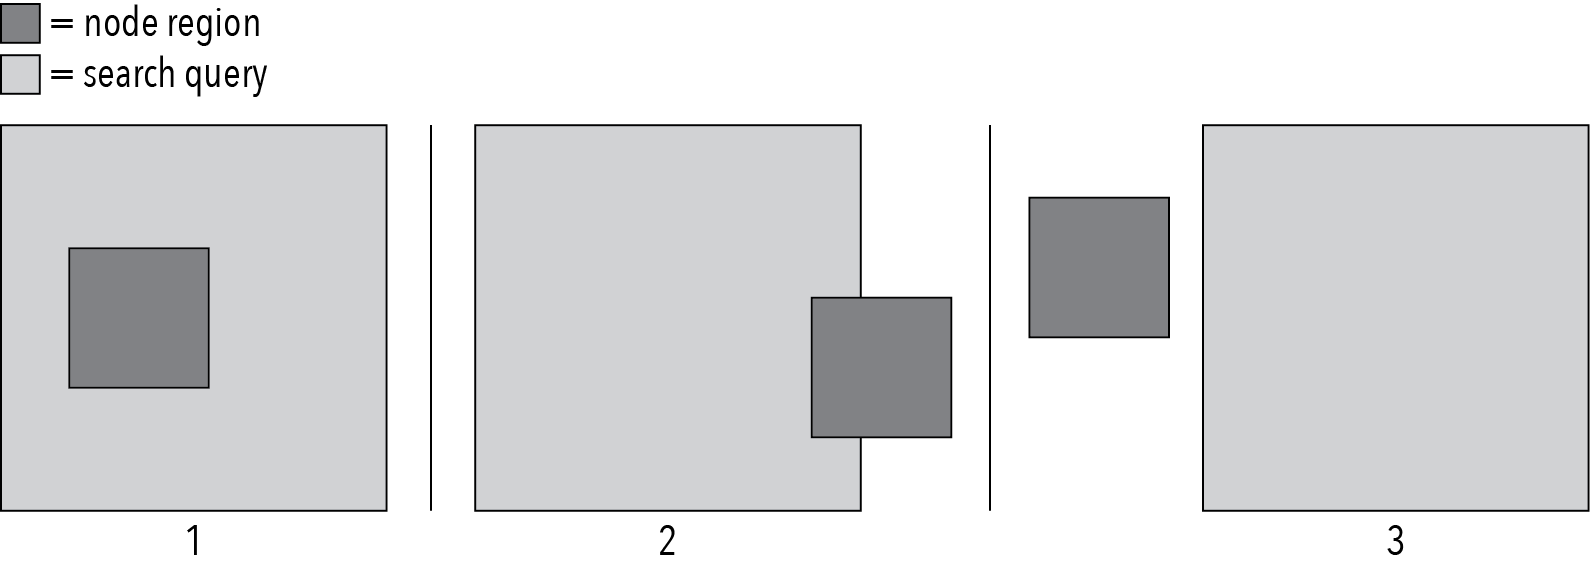
\includegraphics[width = 1.0\textwidth]{pictures/search_query_overlap.png}
    \caption{The three different situations which can occur between a search query and the region of a node}\label{fig:kdsearchoverlap}
\end{figure}

In order to search in this tree, we introduce the term \emph{region}. The region of a node $v$ is the smallest axis-aligned area which contains all the points in the subtree of $v$. The root contains all points and has the biggest region. Since each node contains a line dividing its points between both of its children, we can use this line to decrease the size of the regions of both children. Doing this halves the amount of points lying within each child region. As shown on figure~\ref{fig:kdsearchoverlap}, given an axis-aligned rectangular search query $q = [x_1, x_2] \times [y_1, y_2]$ and a node in the kd-tree one of three things can happen:
\begin{enumerate} 
  \item The region of the node can be fully contained in the search query, in which case the entire node and the points contained in its subtree are returned as part of the result. 
  \item The search query overlaps, but does not fully contain, the region of the node $v$. In this case the search will continue down those children of $v$ whos region overlaps with the search query.
  \item Finally the region of the node and the search query can have nothing in common in which case the search at that node stops. This check will be done by the parent of the node before recursing into the node. 
\end{enumerate}

\todo{Indtil nu - skrives der så rigtigt? Er alt konsistent omkring brug af ``this node'' og ``the children of the node'' og region?}

\noindent If a leaf is visited in the search, the point stored in the leaf is reported as part of the result if it lies within the search query. Also note that internal nodes of the kd-tree are the root of a smaller kd-tree.

Given a node, the time to report back the points stored in the subtree of that node is linear in the number of points reported. Thus, it takes $\mathcal{O}(k_v)$ time to report back all the $k_v$ points stored in the subtree of a node $v$ which is fully contained in the search region. \\

From figure~\ref{fig:kdsearchoverlap} case 1 takes $\mathcal{O}(k_v)$ time and case 3 takes constant time. In order to find the time of a search query to the kd-tree, we need to obtain a bound on the time of case 2. We need to obtain a bound on the amount of nodes visited which is not fully contained in the search region. These are the nodes where an edge of the search query passes through their regions. Consider a search query where one of the edges passes through the region of the root. This edge can be thought of as infinitely long. Without loss of generality, we pick it to be a horizontal line, as seen on figure~\ref{fig:kd_bound}. \\

\begin{figure}[h]
    \centering
    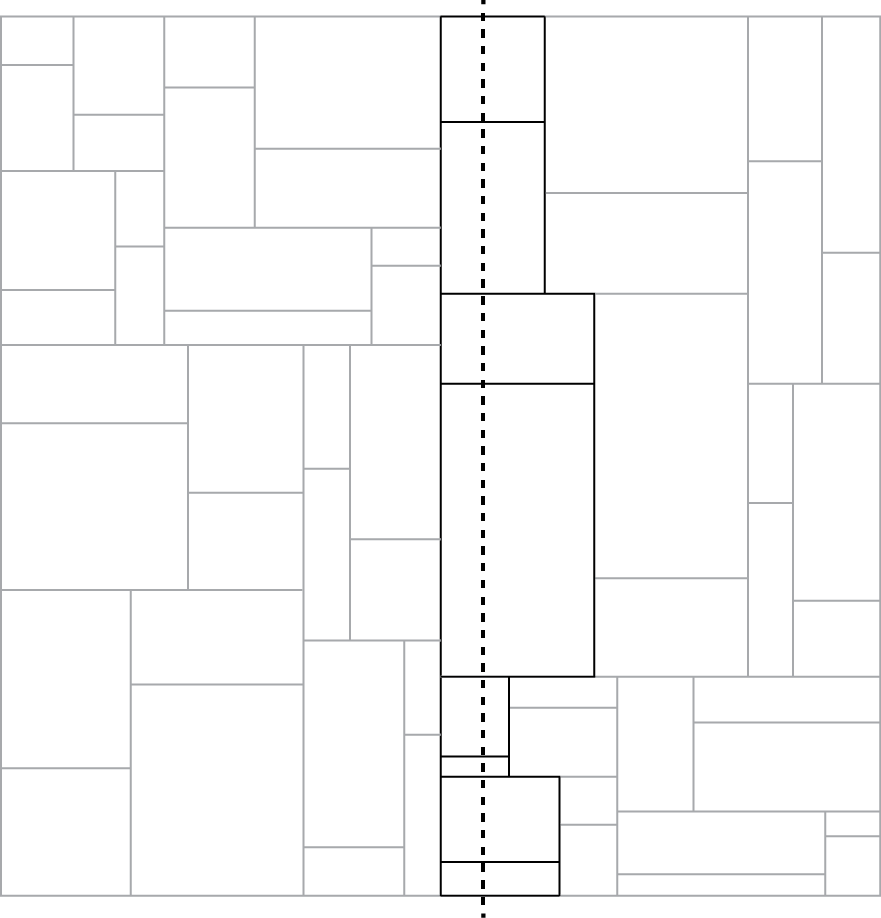
\includegraphics[width = 0.65\textwidth]{pictures/kd_bound2.png}
    \caption{Example of a horizontal edge through the entire region of the root node}\label{fig:kd_bound}
\end{figure}

We want to obtain a bound on the amount of regions this edge can pass through. Let $Q(n)$ describe the amount of regions the horizontal line intersects. In order to find the amount of regions intersected by the line, we need to recall how the kd-tree is built. First a region is split in one dimension and then in the other dimension, resulting in four regions every two levels of the kd-tree constructed \todo{Rephrase sentence - argument should be obvious}. The horizontal line will intersect two of these regions. The horizontal line will also intersect the region of the root and one of the two children of the root. The running time of a query to the kd-tree with $n$ points can be described by the recurrence:

\begin{align*}
  Q(n) = \begin{cases}
    \mathcal{O}(1), & \text{if } n = 1,\\
    2 + 2Q(n/4), & \text{if } n > 1
  \end{cases}
\end{align*}

Solving this recurrence gives the solution $Q(n) = \mathcal{O}(\sqrt{n})$. A horizontal line through the region of the root in a kd-tree will intersect $\mathcal{O}(\sqrt{n})$ regions of the kd-tree, thus bounding the amount of regions of nodes a horizontal line can pass through. The exact same argument can be made for a vertical line.

%% We can also imagine the regions of the kd-tree to form a $m \times m$ grid in the region of the root. Each region in the grid contains one point, and a vertical line through the grid will intersect $m$ regions - one at each row. Since each region in the grid contains a point, we have $m \times m = n$ which gives $m = \sqrt{n}$. Thus, a vertical line through the region of the root will intersect $\sqrt{n}$ regions.

Searching the kd-tree takes $\mathcal{O}(\sqrt{n} + k)$ time to report $k$ points as a result. When the amount of points reported back as result of the search query is low, the query time per point is relatively high. Another thing to notice is that there is no time penalty per point reported. Just searching through the data structure costs $\mathcal{O}(\sqrt{n})$ time, but the time to report back points is linear in the number of points reported.


% The tree with $n$ points can be represented as flat array with $n$ entries. The $\lceil n/2 \rceil$-th element in the array is the root of the tree. \todo{uddyb}

\section{Range trees}
\label{sect:rangetrees}

The range tree is a data structure which supports range queries. The space complexity of this data structure is $\mathcal{O}(n\lg n)$. A normal query in a range tree uses $\mathcal{O}(\lg^2 n + k)$ time to report $k$ points. This time can be optimized to $\mathcal{O}(\lg n + k)$ without changing the space complexity using \emph{fractional cascading}. We will first look at how the data structure is built and how it is used for range reporting. Then we will introduce fractional cascading and see how that will change the query time. With a space complexity of $\mathcal{O}(n \lg n)$ words this data structure is not going to replace the kd-tree. Instead the range tree will serve as a way to introduce some of the ideas behind the SRS and ORS data structures. \\


Consider a balanced binary search tree with $n$ keys for a $1$-dimensional query on the x-coordinates. In order to answer the query $q = [x_1, x_2]$ the following is done: From the root, travel to the \emph{least common ancestor} of $x_1$ and $x_2$. This is the node whose subtree contains both $x_1$ and $x_2$, and $x_1$ lies in the left subtree, while $x_2$ lies in the right subtree. From the least common ancestor, travel to both $x_1$ and $x_2$. While traveling to $x_1$, the first step is the left child of the lowest common ancestor $x_1$ and $x_2$. From here, everytime a left child is chosen as the next step in the path, the subtree in the right child will only contain points between $x_1$ and $x_2$. This entire subtree is reported back as results. Symmetrically, the same is done with the path to $x_2$. When a right child is chosen as the next step, the subtree in the left child is reported back as results. In a $1$-dimensional search, when a node is the root of a subtree which only contains points in the search range, the node is said to be \emph{fully contained}.

A balanced binary search tree has a space complexity of $\mathcal{O}(n)$. Reporting back the points stored in a subtree requires time linear to the amount of points in the subtree. Travelling from the root to $x_1$ and $x_2$ requires $\mathcal{O}(\lg n)$ time. Hence, the query time of a $1$-dimensional search query is $\mathcal{O}(\lg n + k)$.

Range reporting in a $2$-dimensional space on the kd-tree is done by using $1$-dimensional sub-queries. The kd-tree alternates in which dimension the search is performed. The range tree also searches by using $1$-dimensional sub-queries, but instead of alternating between dimensions, it separates them. Given a search query $q = [x_1, x_2] \times [y_1, y_2]$, it will first find the points lying in the range of $[x_1, x_2]$. Among those points, it will find the points lying in the range of $[y_1, y_2]$. This leaves us with all the points lying in the search query.

Doing the first $1$-dimensional search is exactly what is accomplished using a balanced binary search tree. A balanced binary search tree is built to support range search on the x-axis of all of the points. We will call this tree the primary tree. Then for each internal node in the primary tree a new balanced binary search tree is built on all points in the leaves of the subtree of that node. We call these balanced binary search trees for auxiliary trees. The primary tree holds pointers to the auxillary tree for each node.

A range query $q = [x_1, x_2] \times [y_1, y_2]$ on the range tree is answered in the following way. From the least common ancestor of $x_1$ and $x_2$, the search travels down to $x_1$ and $x_2$. On the way to $x_1$ and $x_2$, each node that is fully contained in $[x_1, x_2]$ will be flagged. Using the auxilliry tree of each node that is flagged, a search will be done to find the points in the range $[y_1, y_2]$.

The height of a balanced binary search tree containing $n$ points is $\lg n$. Each point $p$ in the primary tree is only stored in the auxillary trees of nodes on the path to the leaf containing the point $p$. This means that each point $p$ is only stored once per level in the primary tree. Each auxillary tree uses space linear to the amount of points it holds. Thus, the space complexity of a range tree is bounded by $\mathcal{O}(n \lg n)$.

The query time for each auxillary tree that is searched is $\mathcal{O}(\lg n + k_v)$, where $k_v$ is the amount of points that is reported back by the auxillary tree at the node $v$ in the primary tree. The amount of auxillary trees which will be searched is bounded by the length of the path from the least common ancestor of $x_1$ and $x_2$ to the leaves containing $x_1$ and $x_2$. This path can at most visit two nodes per level of the primary tree, and the length is thus bounded by $\mathcal{O}(\lg n)$. The query time of a range search in the range tree is then 

\begin{align*}
  \sum\limits_{v} \mathcal{O}(\lg n + k_v) = \mathcal{O}(\lg^2 n + k)
\end{align*}

\noindent where $v$ are the nodes flagged on the path to $x_1$ and $x_2$ from their least common ancestor. \\

Fractional cascasding can be used to speed up the query time without changing the space complexity of the data structure. Instead of using a balanced binary search tree as the auxillary data structure, we are going to use an array. This array will contain the same points as the auxillary balanced binary search tree did. The points in the array will be sorted by their y-coordinate. At the node $v$, each entry in the array $A_v$will contain a point and two pointers. One pointer will be pointing to an entry in the auxillary array of the left child of $v$, while the other pointer will be pointing to an entry in the auxillary array of the rigth child of $v$. We call these the left pointer and the right pointer, respectively. Suppose that $A_v[i]$ stores a point $p$. Then the left pointer at $A_v[i]$ will be pointing to the first entry in the left childs auxillary array containing a point with a y-coordinate greater or equal to $p_y$. The same applies to the right pointer of $A_v[i]$, pointing to the right child instead of the left child. \\

\begin{figure}[h]
    \centering
    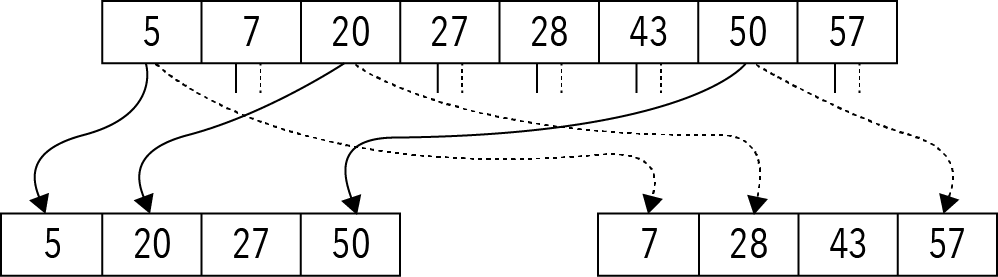
\includegraphics[width = 0.95\textwidth]{pictures/fractional_cascading.png}
    \caption{Example of an fractional cascading}\label{fig:fractional}
\end{figure}


Searching the range tree with fractional cascasding starts by finding the least common ancestor of $x_1$ and $x_2$. At this node, a binary search is done in order to find the first entry in the auxillary array which y-coordinate is greater or equal to $y_1$. At any given node, we call the position of this entry $\tau$. We walk from the least common ancestor of $x_1$ and $x_2$ to both $x_1$ and $x_2$, finding all the nodes which are fully contained in $[x_1, x_2]$. Each time a left child is visited on the path to $x_1$ or $x_2$, the left pointer is used to update $\tau$. The entry at position $\tau_v$ is the first element in $A_v$ which is greater or equal to $y_1$. Finding the index of this element at a child-node is a constant-time operation using the left pointer. Symmetrically, when a right child is visited on the path to $x_1$ and $x_2$, the position of $\tau$ is updated using the right pointer. This can be seen on figure~\ref{fig:fractional} When a fully contained node is found, we look in the auxillary array from the position of $\tau$ and $k_v$ entries forward in order to report $k_v$ points back as result. This is done by incrementing the position of $\tau$ until the point at that entry is no longer within the range of $[y_1, y_2]$. This takes $\mathcal{O}(1+k_v)$ time. The total query time now becomes

\begin{align*}
  \sum\limits_{v} \mathcal{O}(1 + k_v) = \mathcal{O}(\lg n + k)
\end{align*}

\noindent where $v$ are the nodes flagged on the path to $x_1$ and $x_2$ from their least common ancestor.

\section{Composite-number space} 
\label{sect:composite}
In order to ensure all points have unique x-coordinates and unique y-coordinates, the points are translated into \emph{composite-number space}\cite{compgeo}. A composite number of two numbers $x$ and $y$ is denoted by $(x \mid y)$. A total ordering on the composite-number space is defined by using lexicographic order. Given two composite numbers $(x_1 \mid y_1)$ and $(x_2 \mid y_2)$, we define the order as
\begin{align*}
  (x_1 \mid y_1) < (x_2 \mid y_2) \iff x_1 < x_2 \text{ or } (x_1 = x_2 \text{ and } y_1 < y_2)
\end{align*}

\noindent Given a set P of $n$ distinct points from $\mathbb{R}^2$, we translate each point $(x,y) \in P$ into composite-number space by assigning the point new set of coordinates: $(x,y) := ( (x \mid y), (y \mid x) )$. No two points will have the same x-coordinate unless the points are identical. The same holds for the y-coordinate.

\noindent In order to perform a range query $q = [x_1, x_2] \times [y_1, y_2]$ in composite-number space, the query will have to be transformed. This transformed range query will be $\hat{q} = [(x_1 \mid -\infty), (x_2 \mid +\infty)] \times [(y_1 \mid -\infty), (y_2 \mid +\infty)]$. It follows that 
\begin{align*}
  (x,y) \in q \iff ( (x \mid y), (y \mid x) ) \in \hat{q}
\end{align*}


\section{Summary}
\label{sect:relsummary}

The kd-tree is a data structure using $\mathcal{O}(n)$ words of space and supports a range query in $\mathcal{O}(\sqrt{n} + k)$ time. It is built by continually subdividing smaller and smaller regions of the tree until a region only contains one point. A range search query will then match the query region to the region of node to see if there is any overlap or full containment. 

The range tree is a data structure using $\mathcal{O}(n \lg n)$ words of space and support a range query in $\mathcal{O}(\lg n + k)$ time. It is built by creating a tree with $n$ leaves and dividing the points to the leaves, such that all the leaves to the left of a leaf contain points with a smaller x-coordinate than the point at the leaf. All the internal nodes of the tree contain an auxillary tree which has the same property just with the y-coordinate of the points contained in the subtree. This property allows a search query to quickly locate the subtrees containing only points between $[x_1, x_2]$ and $[y_1, y_2]$.

The $\mathcal{O}(\lg n + k)$ running time of the range tree is faster than the $\mathcal{O}(\sqrt{n} + k)$ running time of the kd-tree. However, the $\mathcal{O}(\sqrt{n})$ part is based on a rather pessimistic idea that a range query will overlap, but not fully include, a lot of regions stretching over the two extrema in one dimension.
